\chapter{Anexo}

\section{simulaciones}

  \begin{figure}[H]
    \centering
    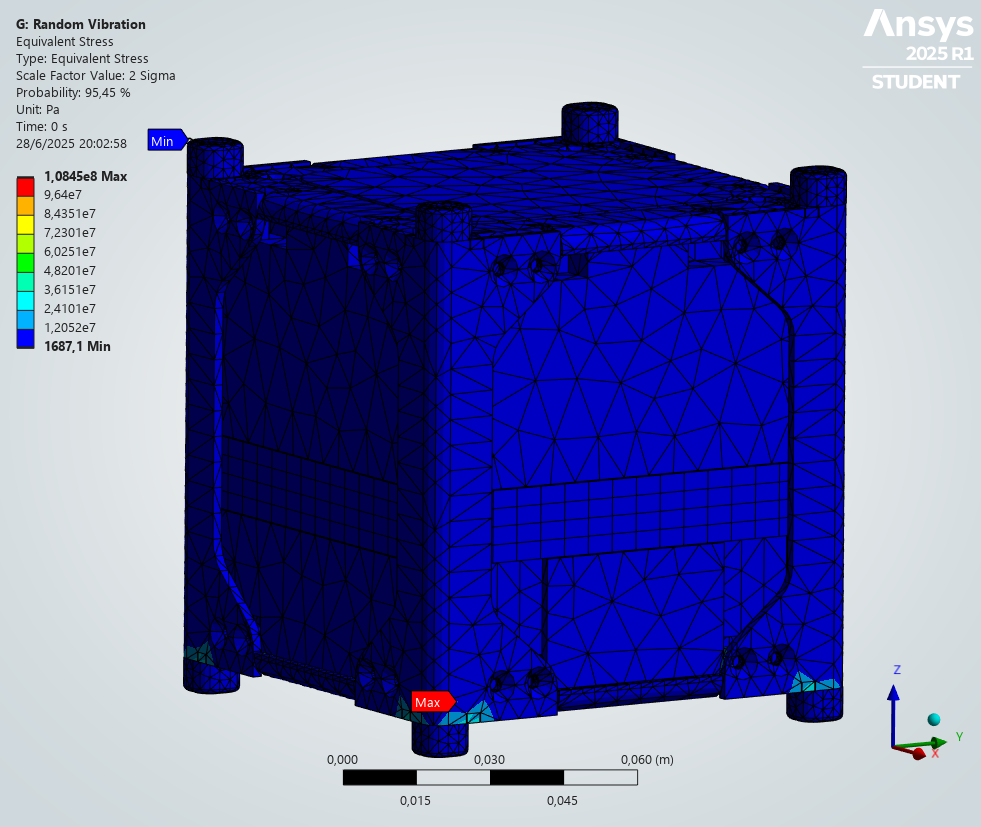
\includegraphics[width=\textwidth]{image/fem/ansys_cubesat-vibration_stress.png}
    \caption{Analisis de estres}
    \label{fig:fem_stress}
  \end{figure}

  \begin{figure}[H]
    \centering
    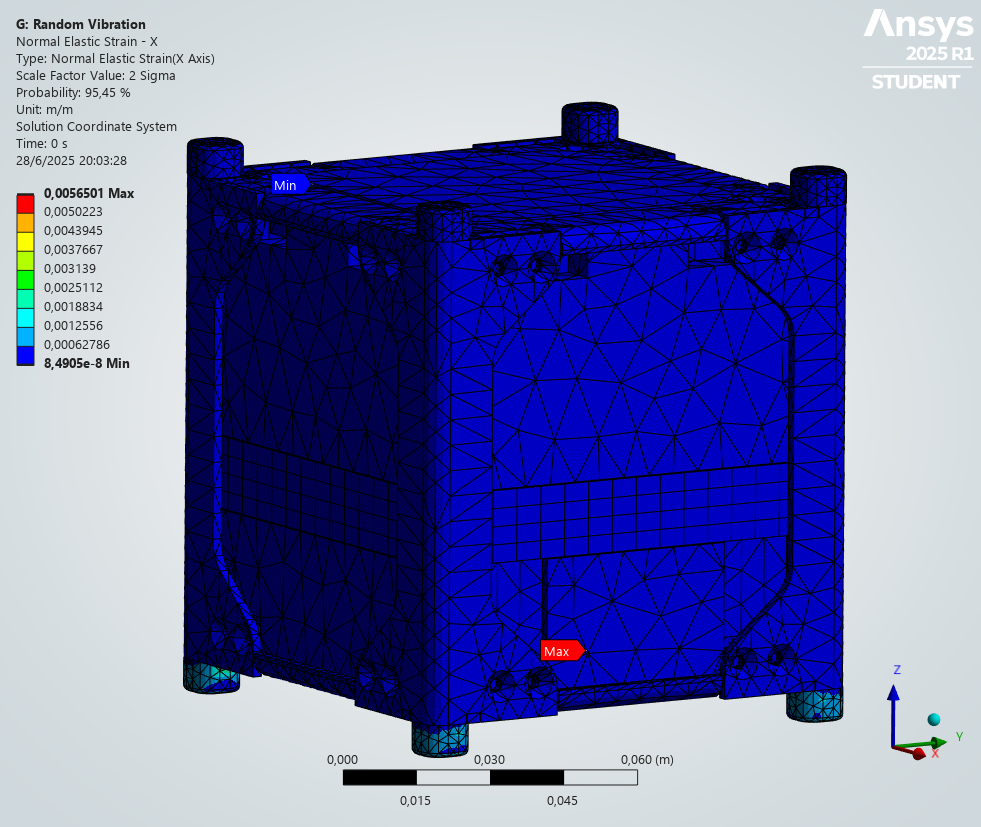
\includegraphics[width=\textwidth]{image/fem/ansys_cubesat-vibration_strain-x.png}
    \caption{Analisis de tensión en el eje x}
    \label{fig:fem_strain-x}
  \end{figure}

  \begin{figure}[H]
    \centering
    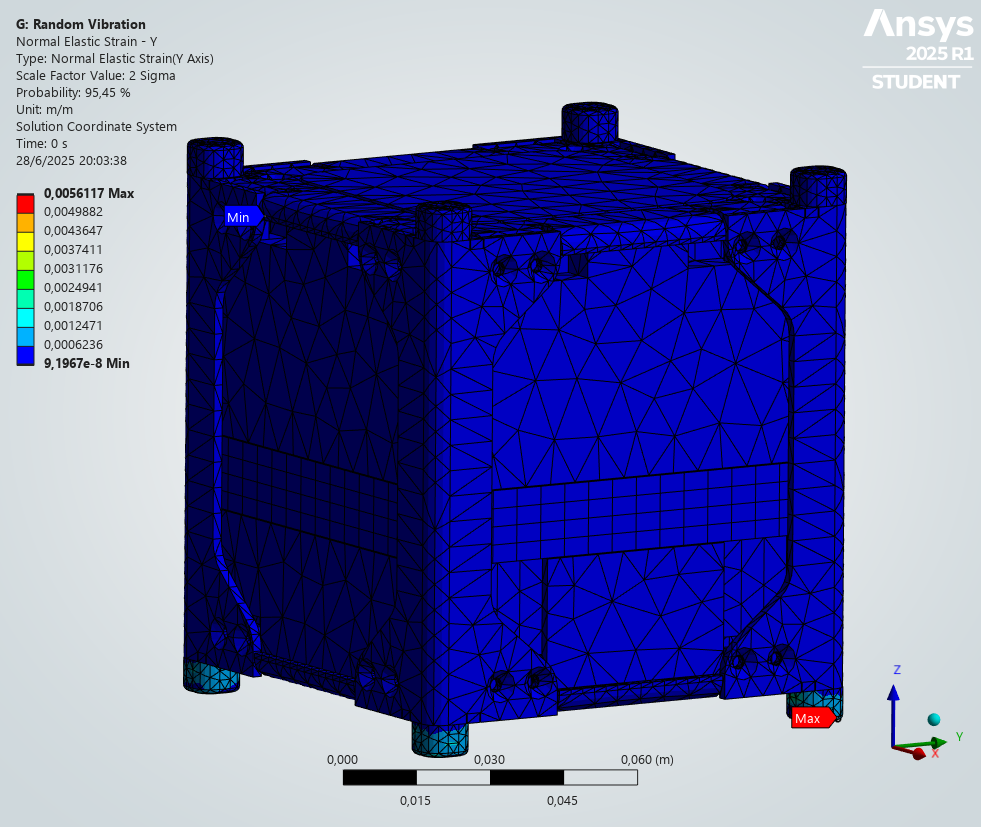
\includegraphics[width=\textwidth]{image/fem/ansys_cubesat-vibration_strain-y.png}
    \caption{Analisis de tensión en el eje Y}
    \label{fig:fem_strain-y}
  \end{figure}

  \begin{figure}[H]
    \centering
    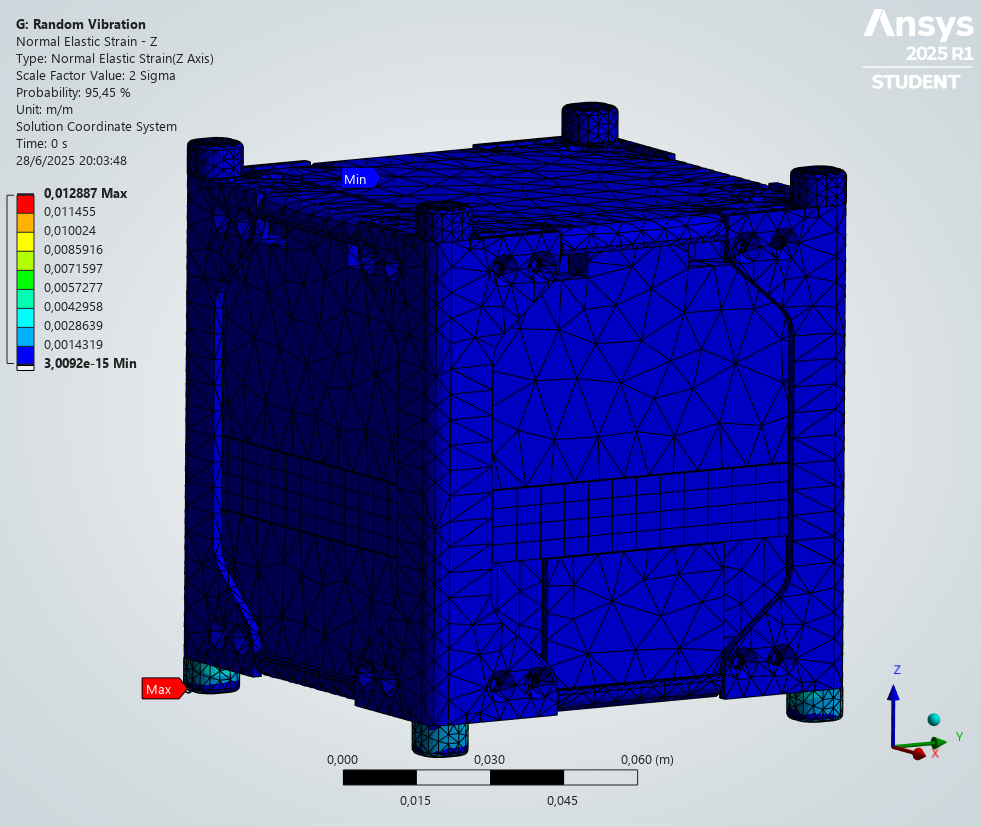
\includegraphics[width=\textwidth]{image/fem/ansys_cubesat-vibration_strain-z.png}
    \caption{Analisis de tensión en el eje Z}
    \label{fig:fem_strain-z}
  \end{figure}

  \begin{figure}[H]
    \centering
    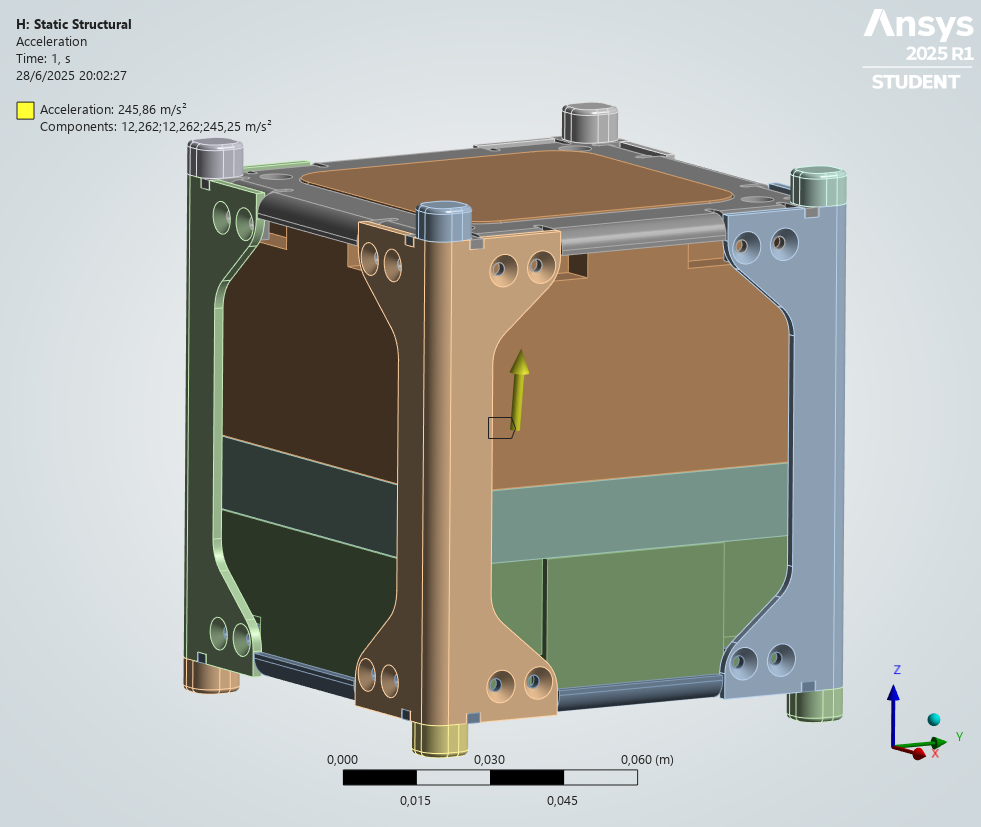
\includegraphics[width=\textwidth]{image/fem/ansys_cubesat-static_acceleration.png}
    \caption{Vector de aceleración para la simulación estática.}
    \label{fig:fem_static_acc}
  \end{figure}

  \begin{figure}[H]
    \centering
    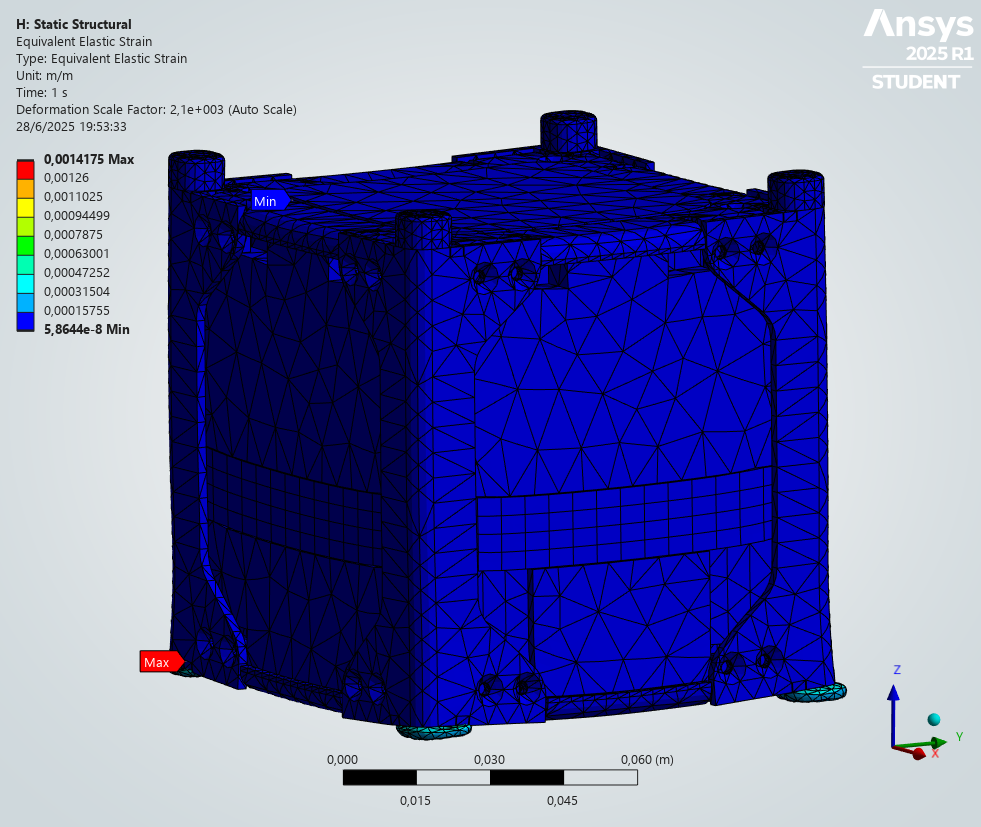
\includegraphics[width=\textwidth]{image/fem/ansys_cubesat-static_strain.png}
    \caption{Analisis de fatiga}
    \label{fig:fem_static_strain}
  \end{figure}

  \begin{figure}[H]
    \centering
    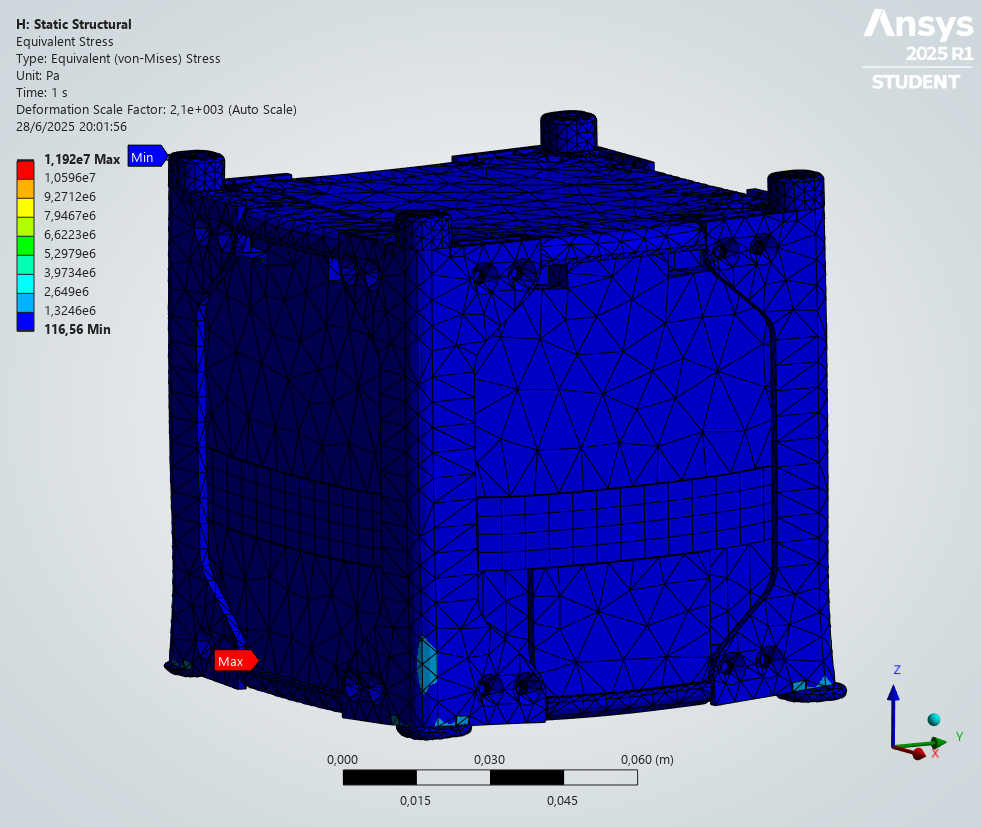
\includegraphics[width=\textwidth]{image/fem/ansys_cubesat-static_stress.png}
    \caption{Analisis de estrés}
    \label{fig:fem_static_stress}
  \end{figure}

  \begin{figure}[H]
    \centering
    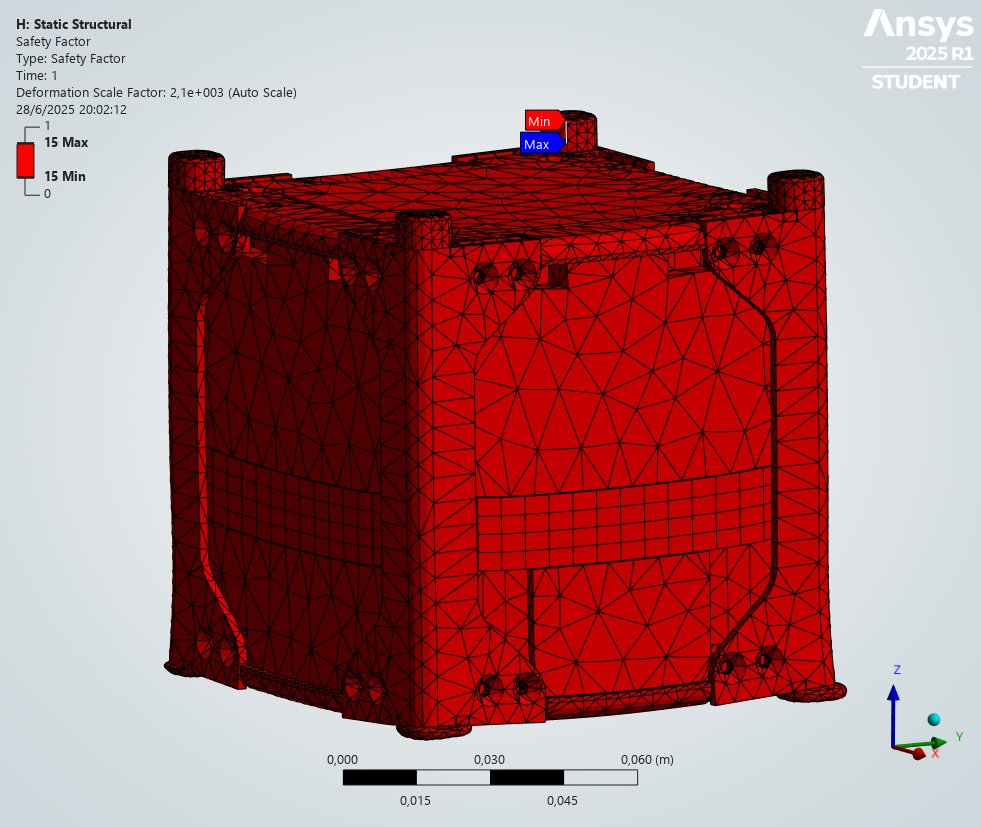
\includegraphics[width=\textwidth]{image/fem/ansys_cubesat-static_safety.png}
    \caption{Analisis de factor de seguridad}
    \label{fig:fem_static_safety}
  \end{figure}

  \begin{figure}[H]
    \centering
    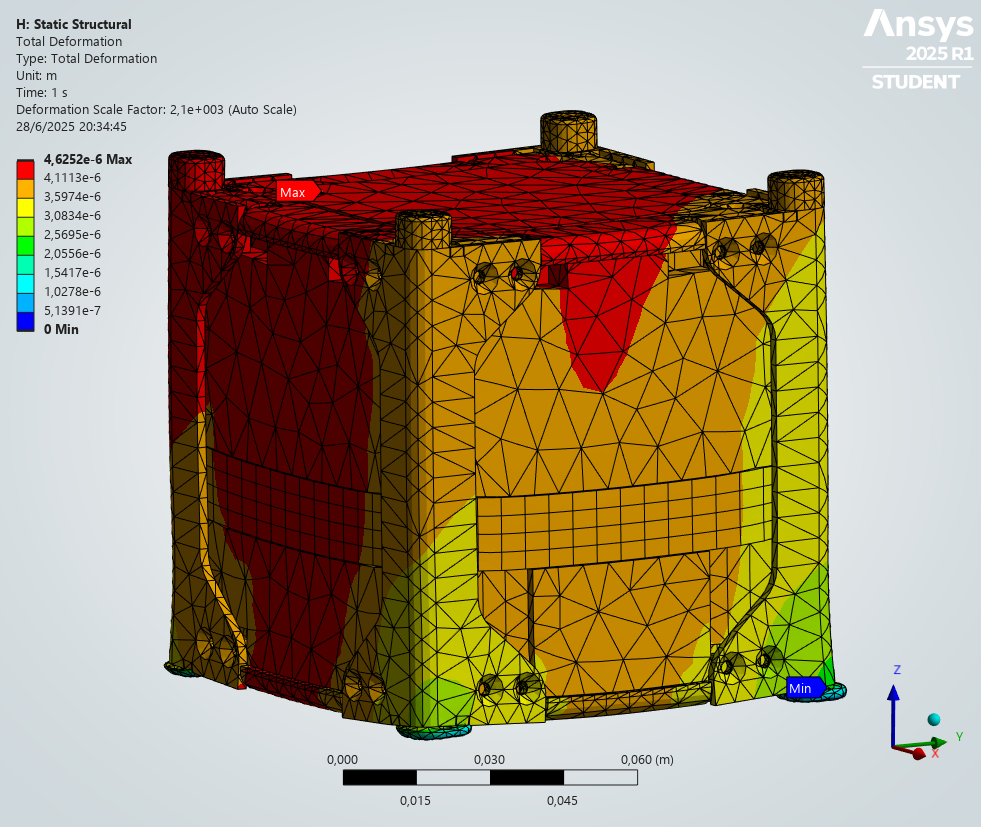
\includegraphics[width=\textwidth]{image/fem/ansys_cubesat-static_deformation.png}
    \caption{Analisis de deformación total}
    \label{fig:fem_static_deformation}
  \end{figure}

\pagestyle{empty}
\newgeometry{left=3mm,right=3mm,top=3mm,bottom=3mm,}
\begin{landscape}
\section{Cronograma Electrónica}

  \resizebox{245mm}{!}{
  \begin{tikzpicture}
  \begin{ganttchart}[
      hgrid,
      vgrid,
      time slot format=isodate,
      time slot unit=day,
      calendar week text={Week \currentweek},
      title/.append style={draw=none, fill=none},
      title label font=\bfseries\footnotesize,
      title label anchor/.style={below=-1.6ex},
      bar/.append style={fill=blue!30},
      progress label text={},
      group right shift=0,
      group top shift=.6,
      group height=.3,
      group peaks height=.2
    ]{2025-07-01}{2025-08-31}

  % July
  \gantttitlecalendar{month=name,week,day} \\

  % Tasks
  \ganttgroup{Validación de Subsistemas}{2025-07-01}{2025-07-12} \\
  \ganttbar{Revisión de PCB}{2025-07-01}{2025-07-06} \\
  \ganttbar{Revisión de Sensores}{2025-07-03}{2025-07-12} \\

  \ganttgroup{CAD Computadora de Vuelo}{2025-07-07}{2025-07-27} \\
  \ganttbar{Diseño esquemático}{2025-07-07}{2025-07-13} \\
  \ganttbar{Diseño PCB}{2025-07-11}{2025-07-18} \\
  \ganttmilestone{Team Meeting}{2025-07-14} \\
  \ganttbar{CAD PMS}{2025-07-15}{2025-07-26} \\

  \ganttgroup{CAD TRU}{2025-07-20}{2025-08-02} \\
  \ganttbar{Diseño esquemático}{2025-07-20}{2025-07-25} \\
  \ganttbar{Diseño PCB}{2025-07-23}{2025-07-30} \\
  \ganttmilestone{Team Meeting}{2025-07-28} \\

  \ganttgroup{Prototipo Mínimo Funcional}{2025-07-30}{2025-08-06} \\
  \ganttbar{Armado}{2025-07-30}{2025-08-06} \\
  \ganttmilestone{Entrega CDR}{2025-08-06} \\

  \ganttgroup{Construcción 1ra versión}{2025-08-07}{2025-08-18} \\
  \ganttbar{Planchado de PCBs}{2025-08-07}{2025-08-08} \\
  \ganttbar{Soldado de componentes}{2025-08-09}{2025-08-10} \\
  \ganttbar{Verificación de test points}{2025-08-10}{2025-08-11} \\
  \ganttbar{Interconexión de sistemas}{2025-08-12}{2025-08-14} \\
  \ganttbar{Identificación de errores}{2025-08-14}{2025-08-18} \\

  \ganttgroup{Construcción Producto Final}{2025-08-19}{2025-08-31} \\
  \ganttbar{Planchado de PCB}{2025-08-19}{2025-08-20} \\
  \ganttbar{Soldado}{2025-08-20}{2025-08-22} \\
  \ganttbar{Funcionamiento en conjunto}{2025-08-22}{2025-08-27} \\
  \ganttbar{Identificación de posibles fallas}{2025-08-27}{2025-08-31} \\

  \end{ganttchart}
  \end{tikzpicture}
  }

\chapter{Anexo}

\section{Simulaciones}

\section{Cronogramas}


  \newpage
      
  \section{Cronograma software}
    \begin{figure}[H]
      \centering
      \resizebox{25cm}{!}{%
        \begin{ganttchart}[
        hgrid,
        vgrid,
        time slot format=isodate,
        x unit=0.65cm,
        y unit chart=0.65cm,
        bar/.append style={fill=blue!40},
        milestone/.append style={fill=orange},
        milestone label font=\bfseries\small,
        bar label font=\small\slshape
    ]{2025-07-05}{2025-08-17}
  
      \gantttitlecalendar{month=name, week, day} \\
  
      \ganttlink{req}{tools}
      \ganttlink{tools}{design}
      \ganttlink{design}{developpdr}
      \ganttlink{developpdr}{delivpdr}
  
      \ganttgroup{Planning}{2025-07-05}{2025-07-05} \\
  
      \ganttgroup{Desarrollo de CDR}{2025-07-08}{2025-08-08} \\
      \ganttbar{Evaluación y revisión de correcciones}{2025-07-08}{2025-08-07} \\
      \ganttbar{Desarrollo de CDR}{2025-07-08}{2025-08-07} \\
      \ganttlinkedmilestone[name=delivcdr]{Entrega de CDR}{2025-08-08} \\
  
      \ganttgroup{Selección de equipo}{2025-08-09}{2025-08-14} \\
      \ganttbar{Evaluación}{2025-08-09}{2025-08-13} \\
      \ganttbar{Selección}{2025-08-14}{2025-08-14} \\
  
      \ganttgroup{Diseño de software}{2025-07-06}{2025-07-09} \\
      \ganttbar{Especificación de funcionalidades}{2025-07-06}{2025-07-09} \\
      \ganttbar{Diseño del sistema}{2025-07-06}{2025-07-09} \\
  
      \ganttgroup{Configuración de entorno}{2025-07-10}{2025-07-19} \\
      \ganttbar{Configuración del sistema operativo}{2025-07-10}{2025-07-14} \\
      \ganttbar{Instalación de herramientas}{2025-07-10}{2025-07-14} \\
      \ganttbar{Configuración de acceso}{2025-07-13}{2025-07-19} \\
  
      \ganttgroup{Integración de sensores}{2025-07-20}{2025-07-24} \\
      \ganttbar{Integración con lectura de sensores}{2025-07-20}{2025-07-22} \\
      \ganttbar{Compresión de datos}{2025-07-23}{2025-07-24} \\

      \ganttgroup{Sprint 1}{2025-07-25}{2025-08-17}\\
      
      \ganttgroup{Desarrollo backend}{2025-07-25}{2025-08-13} \\
      \ganttbar{Desarrollo de funcionalidades principales}{2025-07-25}{2025-07-31} \\
      \ganttbar{Análisis de datos}{2025-07-28}{2025-08-03} \\
      \ganttbar{Generación de reportes}{2025-08-04}{2025-08-08} \\
      \ganttbar{Manejo de errores}{2025-08-09}{2025-08-13} \\
      \ganttbar{Administración de logs}{2025-08-09}{2025-08-13} \\
  
      \ganttgroup{Almacenamiento}{2025-07-27}{2025-08-02} \\
      \ganttbar{Almacenamiento de datos}{2025-07-27}{2025-08-02} \\
      \ganttbar{Implementación RAID 1}{2025-07-27}{2025-08-02} \\
  
      \ganttgroup{Desarrollo frontend}{2025-08-04}{2025-08-10} \\
      \ganttbar{Interfaz visual}{2025-08-04}{2025-08-10} \\
  
      \ganttgroup{Testing}{2025-08-14}{2025-08-17} \\
      \ganttbar{Pruebas unitarias funcionales}{2025-08-14}{2025-08-15} \\
      \ganttbar{Pruebas unitarias no funcionales}{2025-08-14}{2025-08-15} \\
      \ganttbar{Pruebas de estrés}{2025-08-14}{2025-08-15} \\
      \ganttbar{Validación de hardware}{2025-08-16}{2025-08-17} \\
      \ganttbar{Corrección de posibles fallos}{2025-08-14}{2025-08-17} \\
  
    \end{ganttchart}
    }
    \end{figure}

  \newpage
  \section{Cronograma software}
    \begin{figure}[H]
      \centering
      \resizebox{25cm}{!}{%
        \begin{ganttchart}[
        hgrid,
        vgrid,
        time slot format=isodate,
        x unit=0.65cm,
        y unit chart=0.65cm,
        bar/.append style={fill=blue!40},
        milestone/.append style={fill=orange},
        milestone label font=\bfseries\small,
        bar label font=\small\slshape
    ]{2025-08-18}{2025-10-10}
  
      \gantttitlecalendar{month=name, week, day} \\
  
      \ganttlink{req}{tools}
      \ganttlink{tools}{design}
      \ganttlink{design}{developpdr}
      \ganttlink{developpdr}{delivpdr}
  

      \ganttgroup{Sprint 2}{2025-08-18}{2025-09-10}\\

      \ganttgroup{Desarrollo backend}{2025-08-18}{2025-09-06} \\
      \ganttbar{Desarrollo de funcionalidades principales}{2025-08-18}{2025-08-24} \\
      \ganttbar{Análisis de datos}{2025-08-21}{2025-08-27} \\
      \ganttbar{Generación de reportes}{2025-08-28}{2025-09-01} \\
      \ganttbar{Manejo de errores}{2025-09-02}{2025-09-06} \\
      \ganttbar{Administración de logs}{2025-09-02}{2025-09-06}\\
  
      \ganttgroup{Almacenamiento}{2025-08-20}{2025-08-26} \\
      \ganttbar{Almacenamiento de datos}{2025-08-20}{2025-08-26} \\
      \ganttbar{Implementación RAID 1}{2025-08-20}{2025-08-26}\\
  
      \ganttgroup{Desarrollo frontend}{2025-08-28}{2025-09-03} \\
      \ganttbar{Interfaz visual}{2025-08-28}{2025-09-03} \\
  
      \ganttgroup{Testing}{2025-09-07}{2025-09-10}  \\
      \ganttbar{Pruebas unitarias funcionales}{2025-09-07}{2025-09-08} \\
      \ganttbar{Pruebas unitarias no funcionales}{2025-09-07}{2025-09-08}  \\
      \ganttbar{Pruebas de estrés}{2025-09-07}{2025-09-08}  \\
      \ganttbar{Validación de hardware}{2025-09-09}{2025-09-10}  \\
      \ganttbar{Corrección de posibles fallos}{2025-09-07}{2025-09-10}  \\
      
      \ganttgroup{Sprint 3}{2025-09-11}{2025-10-04}\\
      
       \ganttgroup{Desarrollo backend}{2025-09-11}{2025-09-20} \\\ganttbar{Desarrollo de funcionalidades principales}{2025-09-11}{2025-09-17} \\
      \ganttbar{Análisis de datos}{2025-09-14}{2025-09-20} \\
      \ganttbar{Generación de reportes}{2025-09-21}{2025-09-25} \\
      \ganttbar{Manejo de errores}{2025-09-26}{2025-09-30} \\
      \ganttbar{Administración de logs}{2025-09-26}{2025-09-30} \\
  
      \ganttgroup{Almacenamiento}{2025-09-13}{2025-09-19} \\
      \ganttbar{Almacenamiento de datos}{2025-09-13}{2025-09-19} \\
      \ganttbar{Implementación RAID 1}{2025-09-13}{2025-09-19} \\
  
      \ganttgroup{Desarrollo frontend}{2025-09-21}{2025-09-27} \\
      \ganttbar{Interfaz visual}{2025-09-21}{2025-09-27} \\
  
      \ganttgroup{Testing}{2025-10-01}{2025-10-04} \\
      \ganttbar{Pruebas unitarias funcionales}{2025-10-01}{2025-10-02} \\
      \ganttbar{Pruebas unitarias no funcionales}{2025-10-01}{2025-10-02} \\
      \ganttbar{Pruebas de estrés}{2025-10-01}{2025-10-02} \\
      \ganttbar{Validación de hardware}{2025-10-03}{2025-10-04} \\
      \ganttbar{Corrección de posibles fallos}{2025-10-01}{2025-10-04} \\
      
      \ganttlinkedmilestone[name=delivcdr]{Entrega final}{2025-10-10}

      \end{ganttchart}
      }
    \end{figure}



\end{landscape}
\restoregeometry
\setCustomPageStyle

holaaaa
